% Options for packages loaded elsewhere
\PassOptionsToPackage{unicode}{hyperref}
\PassOptionsToPackage{hyphens}{url}
%
\documentclass[
]{article}
\usepackage{amsmath,amssymb}
\usepackage{lmodern}
\usepackage{iftex}
\ifPDFTeX
  \usepackage[T1]{fontenc}
  \usepackage[utf8]{inputenc}
  \usepackage{textcomp} % provide euro and other symbols
\else % if luatex or xetex
  \usepackage{unicode-math}
  \defaultfontfeatures{Scale=MatchLowercase}
  \defaultfontfeatures[\rmfamily]{Ligatures=TeX,Scale=1}
\fi
% Use upquote if available, for straight quotes in verbatim environments
\IfFileExists{upquote.sty}{\usepackage{upquote}}{}
\IfFileExists{microtype.sty}{% use microtype if available
  \usepackage[]{microtype}
  \UseMicrotypeSet[protrusion]{basicmath} % disable protrusion for tt fonts
}{}
\makeatletter
\@ifundefined{KOMAClassName}{% if non-KOMA class
  \IfFileExists{parskip.sty}{%
    \usepackage{parskip}
  }{% else
    \setlength{\parindent}{0pt}
    \setlength{\parskip}{6pt plus 2pt minus 1pt}}
}{% if KOMA class
  \KOMAoptions{parskip=half}}
\makeatother
\usepackage{xcolor}
\IfFileExists{xurl.sty}{\usepackage{xurl}}{} % add URL line breaks if available
\IfFileExists{bookmark.sty}{\usepackage{bookmark}}{\usepackage{hyperref}}
\hypersetup{
  pdftitle={Bayesian Hierarchical Model for estimating prehistoric population development on the Swiss Plateau},
  pdfkeywords={keyword 1; keyword 2; keyword 3},
  hidelinks,
  pdfcreator={LaTeX via pandoc}}
\urlstyle{same} % disable monospaced font for URLs
\usepackage[margin=1in]{geometry}
\usepackage{longtable,booktabs,array}
\usepackage{calc} % for calculating minipage widths
% Correct order of tables after \paragraph or \subparagraph
\usepackage{etoolbox}
\makeatletter
\patchcmd\longtable{\par}{\if@noskipsec\mbox{}\fi\par}{}{}
\makeatother
% Allow footnotes in longtable head/foot
\IfFileExists{footnotehyper.sty}{\usepackage{footnotehyper}}{\usepackage{footnote}}
\makesavenoteenv{longtable}
\usepackage{graphicx}
\makeatletter
\def\maxwidth{\ifdim\Gin@nat@width>\linewidth\linewidth\else\Gin@nat@width\fi}
\def\maxheight{\ifdim\Gin@nat@height>\textheight\textheight\else\Gin@nat@height\fi}
\makeatother
% Scale images if necessary, so that they will not overflow the page
% margins by default, and it is still possible to overwrite the defaults
% using explicit options in \includegraphics[width, height, ...]{}
\setkeys{Gin}{width=\maxwidth,height=\maxheight,keepaspectratio}
% Set default figure placement to htbp
\makeatletter
\def\fps@figure{htbp}
\makeatother
\setlength{\emergencystretch}{3em} % prevent overfull lines
\providecommand{\tightlist}{%
  \setlength{\itemsep}{0pt}\setlength{\parskip}{0pt}}
\setcounter{secnumdepth}{5}
\newlength{\cslhangindent}
\setlength{\cslhangindent}{1.5em}
\newlength{\csllabelwidth}
\setlength{\csllabelwidth}{3em}
\newlength{\cslentryspacingunit} % times entry-spacing
\setlength{\cslentryspacingunit}{\parskip}
\newenvironment{CSLReferences}[2] % #1 hanging-ident, #2 entry spacing
 {% don't indent paragraphs
  \setlength{\parindent}{0pt}
  % turn on hanging indent if param 1 is 1
  \ifodd #1
  \let\oldpar\par
  \def\par{\hangindent=\cslhangindent\oldpar}
  \fi
  % set entry spacing
  \setlength{\parskip}{#2\cslentryspacingunit}
 }%
 {}
\usepackage{calc}
\newcommand{\CSLBlock}[1]{#1\hfill\break}
\newcommand{\CSLLeftMargin}[1]{\parbox[t]{\csllabelwidth}{#1}}
\newcommand{\CSLRightInline}[1]{\parbox[t]{\linewidth - \csllabelwidth}{#1}\break}
\newcommand{\CSLIndent}[1]{\hspace{\cslhangindent}#1}
\ifLuaTeX
  \usepackage{selnolig}  % disable illegal ligatures
\fi

\title{Bayesian Hierarchical Model for estimating prehistoric population development on the Swiss Plateau}
\author{true \and true \and true \and true \and true}
\date{07 April, 2022}

\begin{document}
\maketitle
\begin{abstract}
In order to understand human-environment relationships in the past and the dynamics of socio-ecological systems, it is essential to have a robust estimate of population sizes. Size and density of population are crucial factors for the reconstruction of group sizes, the character and range of political institutions for social organization, the constraints and possibilities of economic practice, the number of people available for collective activities, for economic and social exchange systems, and the creation and maintenance of collective identities. And, of course, the human impact on the environment. Most estimates of population sizes currently work on limited spatial scales or use proxies that hardly allow for absolute numbers (e.g.~sum calibration). The figures in the archaeological discourses on population density in general currently come from vague sources and are often decades old.
In demography in general, the last decade has triggered an upswing in the application of Bayesian methods, so that a Bayesian demography has been announced. Bayesian demography is currently at the forefront of methodological developments in this area, but has reached such maturity that the United Nations has been using it since 2015 for population forecasts and projections. The Bayesian approach offers the possibility of combining heterogeneous data and at the same time qualifying them in terms of uncertainty and credibility. This is precisely where it becomes very interesting for archaeological data, since they are mostly inaccurate, biased, sparse, simplified and often based on simplistic assumptions.
In this contribution, issues and possibilities of the application of Bayesian demography in the field of archaeological (prehistoric) population size and density estimation will be discussed and the results of a pilot study will be presented, which should lead to a more comprehensive project for the reconstruction of demographic developments in prehistory on a large scale.
\end{abstract}

{
\setcounter{tocdepth}{2}
\tableofcontents
}
Keywords: keyword 1; keyword 2; keyword 3

Highlights: These are the highlights.

\hypertarget{introduction}{%
\section{Introduction}\label{introduction}}

The study of population size and population density as important demographic factors has a long history in archaeology. Although questions of population extent and distribution have been dominant fields since the beginning of archaeological research, the lack of access to this information, data on it, or methodological tools for the use of proxies has long made the statements made on this topic for prehistoric times vague and superficial (Hassan, 1981), and they were often based on uncritical transfer of ethnographic parallels.

Gordon Childe (1936) was one of the first to stress the importance of estimating the density and characteristics of prehistoric populations and sought to examine the role of human populations in the course of cultural evolution (Hassan, 1981).

Attempts to estimate the size and density of prehistoric populations from archaeological remains were made by Hack (1942), Colton (1949), Frankfort (1950) and Cook (1946). Cook and Heizer (1965, 1968) and Naroll (1962) provided rules derived from ethnographic contexts for estimating the size of prehistoric populations. Cook and Heizer (1966) made the first attempt to estimate the population growth rate during the Neolithic (Hassan, 1981).

At the end of the 1960s, however, with the emergence of the processual archaeology, such investigations became increasingly popular. It was the rise of the ecological paradigm that gave even greater weight to population studies, especially those dealing with population ecology (Hassan, 1981).

After research interest turned increasingly to other aspects with the emergence of post-process trends, a strong boom in the study of population sizes can be observed especially since the 2010s (or even earlier, (Shennan, 2000)). This is probably due, on the one hand, to the new shift towards the study of human-environment relationships, for which an assessment of the size of human populations is indispensable. This is true especially for an evaluation of the human impact on the natural environment. Another reason is certainly the emergence of the `dates as data' approach (Rick, 1987), which only really took off with the publications around the London UCL group. Moreover, Kintigh et al. (2014) listed human influence, dominance and population size and growth as one of the key elements where methodological improvements are necessary in the article on the Grand Challenges for archaeology, in the area of `human-environment interactions'.

Müller and Diachenko (Müller and Diachenko, 2019) has compiled a list of currently used approaches and proxies for estimating prehistoric population sizes. These can be roughly divided into ethnographic parallels, ecologic-economic deductive estimates, and the counting and spatial interpolation of archaeological features (settlements, houses, individual find types). From this short literature review three basic problems are common to all these approaches and the studies based on them:

\begin{enumerate}
\def\labelenumi{\arabic{enumi}.}
\tightlist
\item
  Proxy is based on a single line of evidence. Although multiproxy approaches exist, in such cases the individual proxies only serve to support each other or the proxy used in the main case. There is no combination of results to increase the accuracy of each of the inaccurate and biased proxies.
\item
  The uncertainty of evidence is not adequately reflected. In most cases, individual curves are presented as estimates, but the size of the error bars for these estimates is almost never apparent.
\item
  Nature of the archaeological data is taken into account only insufficiently. What is meant here is that they take little account of the inherent uncertainties of the proxies themselves, for lack of an evaluative framework, and that transfer functions from the proxy to the actual size to be observed, i.e.~population size or density, are hardly ever evaluated more intensively. In the best case, a critical appraisal of the informative value is provided, but a quantification of the relationship between, for example, a doubling of a proxy value and the change in population density does not take place and cannot take place for lack of a suitable framework or external data for calibration.
\end{enumerate}

\[Beispiele bringen? Bring some examples here...\]

Archaeological data used to estimate population trends have the following characteristics:

\begin{itemize}
\tightlist
\item
  Limited: We have only incomplete data that can be used for these purposes, and they are usually very low in information value.
\item
  Unevenly distributed: Although there is a good data on settlement frequencies for some regions, and these are sometimes in very high temporal resolution, such favorable situations are very unevenly distributed over time and space.
\item
  Noisy: Often other influences, not related to population development, affect the characteristics of individual proxies. Preservation conditions, depositional behavior or social aspects should be mentioned here as an example.
\item
  Unreliable: Comprehensive information and derived data are influenced by research strategies. Systematic distortions are possible or rather the rule.
\item
  Highly heterogeneous: The number of artefacts at a site, the number of houses, the demographic conditions in cemeteries, the estimates of human impact based on pollen analyses: All these are data that may serve our purposes, but which are available in completely different spatio-temporal scales, granularities and information values, and simply represent technically very different data formats and scales.
\item
  Indirect: It is actually always proxy data that are collected as substitute values for the information that is actually needed (i.e.~population density or size). The transfer functions that link the collected data with the data to be obtained are unknown and are at best established by observing the (also ethnological) presence. However, since living conditions, circumstances and economic parameters differ greatly between the present time and prehistory, these transfer functions can only be evaluated as a first approximation.
\item
  Contradicting: Particularly when considering several proxies, differences in transfer functions and data quality and noisiness inevitably lead to contrasts. However, this usually only leads to the rejection of a proxy for a certain time period, without mutually supporting or contradictory information leading to a quantitative evaluation of the proxy and its uncertainties.
\end{itemize}

In recent years, a new method has been established in the field of demographic estimations. Bayesian demographic forecasting has been designed to solve all these problems, which also exist for demographic estimations using recent data. In their book on the subject, Bryant and Zhang \[BrynatandZhang\] state that Bayesian data modeling can be used to deal with exactly those problems that also affect archaeological data. Especially for limited, unreliable and noisy data, Bayesian approaches are optimally suited. Various even contradictory data can be brought into a common framework and support each other. Similarly, unlikelihood and uncertainty of a model approach can be quantified. This is well-accepted in archaeological applications through the Bayesian calibration and modelling of stratigraphic conditions and radiometric data. Furthermore, spatially and temporally missing data can be taken into account: Where these data are missing, the uncertainty automatically increases, but this does not prevent general modelling and estimation. Finally, hierarchically structured model suites, in which sub-models are created for the utilisation of individual proxies, can also be used to estimate transfer functions between individual proxies and the value to be modelled, thanks to the interaction of a large number of data sources and evidence.

Bayesian modelling techniques have also been used recently as a tool for hypothesis testing of demographic trends or underlying models based on 14C data.Most notably are the recently published papers by Crema et al.~However, the approach taken by Crema et al.~is clearly different from the one presented in this paper.In these analyses, deductive models are generated and their plausibility is tested on the basis of 14C data only. This is a clear step in the direction of a model-based, and thus scientific, analysis.However, on the one hand, the use of only one proxy, and its use exclusively for testing hypotheses developed independently, creates problems comparable to those of inductive approaches used so far: due to the lack of a combination with other indicators, one is limited to the problems and conditions of sum calibration as a tool. Furthermore, this approach loses significant potential information that would be gained by a direct evaluation of the time series.Thus, the credibility of a model can only be checked as a whole, without the dynamic developments that can arise in the course of demographic processes being represented. Therefore, we would like to better exploit the capabilities of Bayesian hierarchical models through a combination of inductive data analysis and model-passed data integration of different proxies.

This contribution now represents an attempt to make these techniques usable for archaeological reconstructions. In addition to a presentation of the basics and possible procedures, we want to show in the following, in a reproducible and practical form using a case study, how Bayesian methods can also make a decisive contribution to a better assessment of population development. These assessments are crucial for the reconstruction of the human past, even in for periods for which we only have very patchy, noisy and unreliable data.

\hypertarget{background}{%
\section{Background}\label{background}}

At the heart of all Bayesian statistics is the concept of updating a given prior assumption with new data and expressing this in probabilities (refs.). Our assumptions about the demographic development of the past must naturally be very conservative. In the logic of the basic Bayesian equation, these assumptions represent the prior (probability). In conjunction with the data that are included as the likelihood of the prior, a posterior (probability) results, which represents the Bayesian learning from data. It is also in the nature of the approach that in real applications there is no point prediction, but in most cases a probability distribution for the prediction. Thus we simultaneously obtained a result and an estimate of the confidence intervals, or better, the credibility interval given the data.

This Bayesian learning is iterative and sequential, so that the result of one Bayesian inference can form the prior of another, i.e.~it is an additive process. Moreover, at the conceptual level, this allows different sources of information to be combined. This enables that they can be mapped to the same set and the same real-world domain, e.g.~probabilities. This fact has long been exploited by archaeology in using stratigraphic information to make radiometric dating more accurate. \textsuperscript{14}C dates and stratigraphy are something completely different, but both can be mapped to the probability of older and younger and combined in this way. The same is also conceivable (and feasible) when it comes to the probability of population sizes or population densities or their derived dynamics (increase, decrease).

A further characteristic of Bayesian modeling is that, due to the fact that results of a Bayesian inference can be regarded as a priority for the next one, a hierarchical formulation of problem domains is possible. Parameters that are necessary for an estimation, such as the relationship of population density to the clearing signal in pollen data, need not be specified explicitly, but can be given by probability distributions and then estimated in the model itself. The more data available, the more degrees of freedom can be estimated with a reasonable loss of confidence or a reasonable width of credibility intervals. For the estimation of these parameters, in turn, submodels have to be created which describe the relationship of the data to the characteristics of the parameter. This can be carried out over several levels, depending on necessity.

This modeling technique can thus be used to combine different lines of evidence horizontally and vertically and in this way combine their results into a common conclusion and estimate, which at the same time includes an estimation of their reliability: if the data contradict each other, the overall reliability will be lower. If they support each other, the confidence interval will be smaller. And if there is no systematic bias that affects all data sources to the same extent, it should be possible to arrive at the most reliable estimate possible through the most heterogeneous set of data sources.

A special class of Bayesian hierarchical models are so-called State Space Models (also known as Hidden Markov Models). These are specifically designed for time series and follow two basic principles. First, a hidden or latent process is assumed, which represents the state of the variable of interest \(x_t\) at all times. For the course of the states of this variable over time, it is assumed that every state of variable x in the future, as well as in the past, is bound by a Markov process to the state of variable \(x\) at time \(t\). At the same time, it is assumed that certain observations, represented in variable y, are dependent on the state of variable \(x\) at time \(t\). This means that there is a relationship between the variable \(x\) and the state of variable y over time. This implies that a relationship between the individual states of variable \(y\) is generated over time via the hidden variable \(x\), which itself is not observable.

This basic structure of the model makes it particularly useful and suitable for the purpose of demographic reconstruction using archaeological, but also other data, which depend on population density in the past. This population density itself is not accessible or measurable by our means. All we have at our disposal are observations derived by unknown transfer functions. These can be of very different natures, such as number of archaeologically observable settlements, or other effects that can be observed through time series, and which are influenced by population in a given area. In our example, these are the openness indicators from pollen data, which we can interpret primarily in terms of human influence and its intensity. On a more abstract level, we can also include expert estimates, as these also happen on (often unspecified) bases that are at least indirectly influenced by past population density. The specifics of the individual data we used in this modelling are discussed in the section \ref{dataproxies}.

\hypertarget{methods}{%
\section{Methods}\label{methods}}

\hypertarget{process-model}{%
\subsection{Process Model}\label{process-model}}

The overall model for the estimation of demographic developments is broken down into several hierarchically interconnected individual elements in accordance with the basic structure of a state space model. The basis is a process model that represents the demographic development itself in terms of a structure model, without this model already being explicitly configured with data.

In this process model we assume that the latent variable number of sites is strongly autocorrelated across different time periods. In principle, one can represent a population development in such a way that the population at time \(t\) results from the population at time \(t-1\) times a parameter \(\lambda\), which represents the population change at this time. This results in the following very simple formula:

\[
N_t = N_{t-1} * \lambda_t
\]

A distribution that is particularly suitable for modelling frequencies is the Poisson distribution. It is a univariate discrete probability distribution that can be used to model the number of events that occur independently of each other at a constant mean rate in a fixed time interval or spatial area. It is determined by a real parameter \(\lambda\) \textgreater0, which describes the expected value and simultaneously the variance of the distribution. Thus, the relationship shown above can also be rearranged as follows:

\[
N_t \sim dpois(\lambda_t) \\
\lambda_t = N_t
\]
If we now have information about the change in population development, we can use this to enter it into the model via a change in \(\lambda\). This is done in the form of a regression: If \(x \in R^n\) is a vector of independent variables, then the model takes the form

\[
log({E} (Y\mid x))=\alpha + \beta' x
\]
In the case of population trends, the expected value would be equal to the value of the population in the previous time period, plus or minus the changes resulting from the variables:

\[
log(\lambda_t) = log(N_t) + \sum_{i=1}^n \beta_i x_{t,i}
\]

The values for population size \(N_t\) as well as for population change \(\lambda_t\) are time-dependent. At each individual point in time in the time series, these variables can or will also take on different values. However, we can narrow down the structure of population change even further. We can assume that, considered overall over time, the population change the population change will not exceed certain limits over the entire time span, without it being possible here to specify this already.

Thus, we can define the limits, the \(max\_change\_rate\) as an time independent variable, again without already specifying them with fixed values at this stage. The estimation of these parameters for the entire model, as well as the estimation of the respective population change per time section, results from the modelling and the interaction with the data, respectively. Overall, this represents a hierarchical model that can be noted as follows:

\$\$
max\_growth\_rate \sim dgamma(shape = 5, scale=0.05) \textbackslash{}

N\_t/N\_\{t-1\} \textless{} (max\_growth\_rate + 1) \textbackslash{}
N\_\{t-1\}/N\_t \textless{} (max\_growth\_rate + 1)
\$\$

The gamma distribution used centres the probability in a range \([0,1[\), adding 1 makes this range \([1-2[\) (See also Figure X).

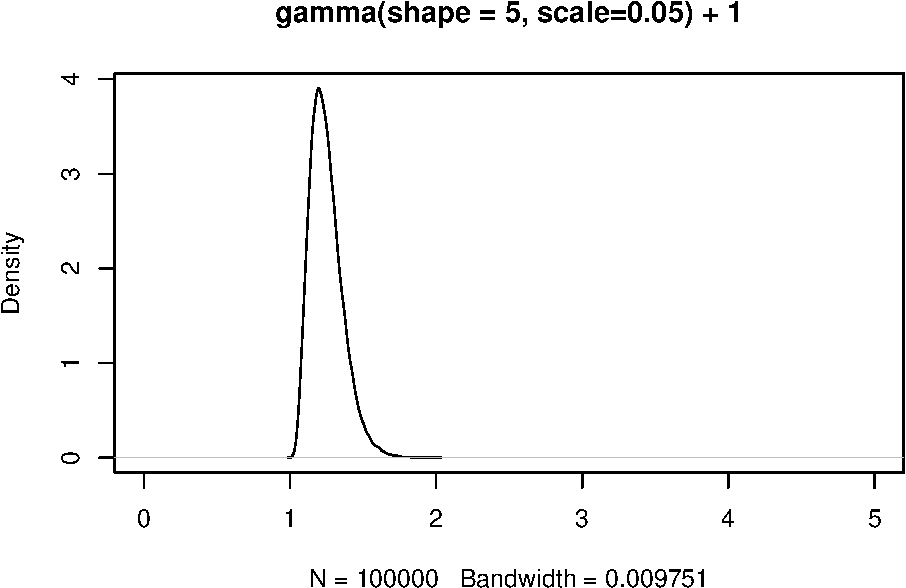
\includegraphics{../figures/unnamed-chunk-1-1.pdf}

This prevents the number of sites from explosively increasing between two time periods, which would lead to problems for the convergence of the model. The interaction of these parameters results in the following prior probability distribution for \(\lambda\) and thus the growth (or change) rate of the population:

\[Prior Probability Simulation einbauen\]

\hypertarget{dataproxies}{%
\subsection{Data/Proxies}\label{dataproxies}}

In principle, a large number of different data sources can be integrated into the overall model as observations, provided that these observations a) can be understood as dependent on the population density in the past, and b) a model-like description of this dependence can be created. A non-exhaustive list can be found in the following table:

\begin{longtable}[]{@{}l@{}}
\caption{(\#tab:table\_proxies) A incomplete list of possible observation that can be linked to population developments in the past. Proxies used in this study are highlighted.}\tabularnewline
\toprule
Proxies \\
\midrule
\endfirsthead
\toprule
Proxies \\
\midrule
\endhead
\textbf{Expert estimates} \\
Ethnographic Analogies \\
Carrying Capacity \\
Economic modelling \\
Extrapolation of buried individuals \\
Burial anthropology \\
Settlement data, number of houses \\
Settlement data, settlement size \\
\textbf{Aoristic analysis} \\
\textbf{Dendro dates} \\
Amount of archaeological objects \\
\textbf{Radiocarbon sum calibration} \\
Estimates based on specific object types \\
\textbf{Human impact from pollen or colluvial data} \\
aDNA based estimates \\
\ldots{} \\
\bottomrule
\end{longtable}

Our working region consists of the Swiss Plateau, which on the one hand offers excellent data for demographic estimation, but on the other hand poses very specific problems for such an undertaking. If we have high-resolution information on the temporal sequence of individual settlements at the lakeside settlements by means of dendro data, this also causes a research problem with regard to the \textsuperscript{14}C data often used as a proxy. Since many periods of the Swiss prehistoric dry land settlements are unknown, and archaeology is based primarily on the wet land settlements, the dendro data are used primarily here, since they are much more precise. As a result, \textsuperscript{14}C data could be largely absent in this time period. If the amount of \textsuperscript{14}C data were now evaluated directly and naively over time, it would show that in the phases of particularly active settlement of the lakeshore, the \textsuperscript{14}C sum calibration shows minima.

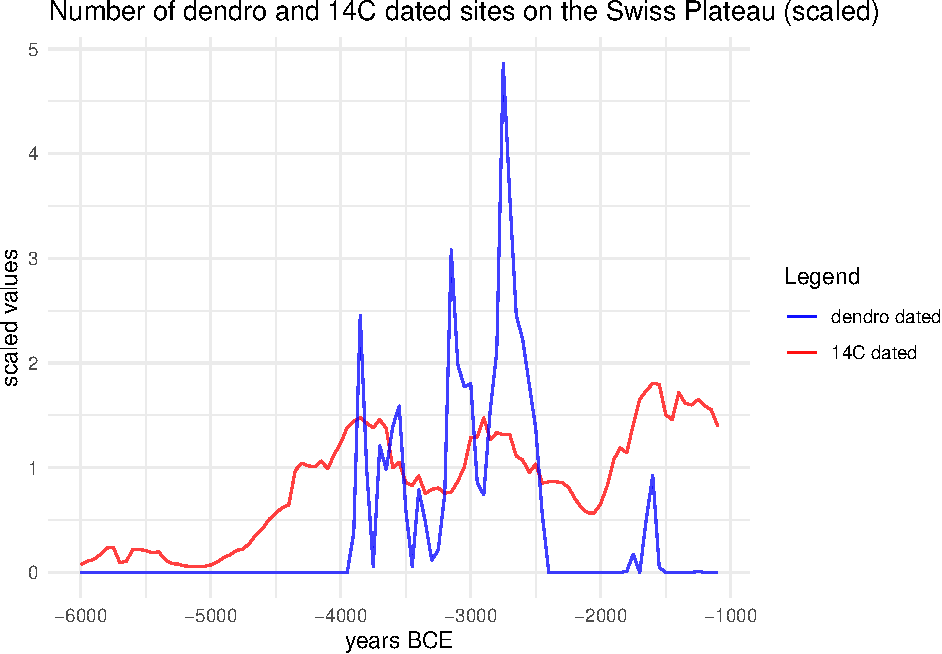
\includegraphics{../figures/unnamed-chunk-2-1.pdf}

In fact, there is a not uninteresting fit between the two data series. However, it must be assumed that the two dating methods, even if they would contradict each other, actually complement each other, and thus allow a better overall unified picture of the actual settlement density than each of the individual proxies would allow on their own.

We have integrated the \textsuperscript{14}C data as one of the proxies in the model, in the form of a sum calibration. The dataset consists of 1135 \textsuperscript{14}C dates from 246 sites, and dates between 10730 and 235 BP uncal. We binned the data at site levels to obtain a temporally dispersed count and thus an expected value of contemporaneous \textsuperscript{14}C dated sites. For the creation of the cumulative calibration, the corresponding functions of the R package rcarbon {[}!citation!{]} were used in the standard settings.

\[Histogramm 14C Datierungen\]

Zugleich stand uns ein Datensatz über die Anzahl der Dendrodatierten Feuchtbodensiedlungen in der Drei-Seen-Region zur Verfügung, welcher durch Julian Laabs für seine PhD-These gesammelt worden ist und deren Hintergrunddaten am genannten Ort veröffentlicht werden. Die hier verwendete Zeitreihe läuft von X bis Y, und enthält die Anzahl von zeitliche verzeichneten Schlagphasen an einzelnen Siedlungen. Somit ergibt sich hier eine Zeitreihe, die die Besiedlung der Seeufer in der Zeit des Neolithikums und der Bronzezeit (?) wiederspiegelt.

In order to add another indicator of archaeological evidence of occupation, we have included the data of the Cantonal Archaeology, and thus the Heritage Management, which are primarily derived from scattered surface finds, and which often have a low depth of information and thus dating accuracy. This information is incorporated into our model as a typologically dated aorist time series. Although the dating accuracy is very low, the advantage here lies in the fact that we are not bound to the conditions and problems of radiocarbon dates, and thus involved in the issue of sum calibration. Much more, these data provide an independent indicator with regard to the methodology of the \textsuperscript{14}C data, even if they are influenced by the same transmission filters and archaeological conditions as the evaluation of \textsuperscript{14}C data. Data from x sites were included in the aoristic sum, which is a very rough indicator due to the low dating accuracy in archaeological phases, but which nevertheless has an important role in the normalisation of the data due to its independence from calibration effects.

\[Abbildung Aoristische Kurve\]

Die durch die vielen sehen Natur räumlich gegebenen Gegebenheiten ermöglichen neben einer hoch präzisen Datierung von archäologischen Fundstellen gleichzeitig aber auch ein sehr dichtes Netz an pollenanalytischen Untersuchungen. Diesen Fakt machen wir uns zu Nutze, in dem wir aus den Pollendaten einem überregionalen Offenheitsanzeiger für den Bewuchs generieren. Genaueres dazu wird im Methoden Kapitel ausgeführt. Dieser Indikator hat spezifisch den Vorteil, dass er nicht an Überlieferungsbedingungen gebunden ist, wie ist die archäologischen Indikatoren sind. Damit wird er besonders wertvoll, um systematische Verzierungen anzuzeigen oder auszugleichen, die sich durch zeitlich spezifische Siedlungsweisen und Überlieferungsbedingungen ergeben.

Es ist eine allgemein akzeptierte Annahme, dass der menschliche Einfluss umso größer ist, je höher die Bevölkerungsdichte in einem Gebiet ist (Lechterbeck et al.~2014), und dass die Bevölkerungsdichte eines Gebiets eng mit der landwirtschaftlichen Fläche zusammenhängt (Zimmermann et al.~2004). Hinweise auf Landrodung in Pollendiagrammen können daher zusätzliche Anhaltspunkte für die Bevölkerungsdynamik liefern. Da ein einzelnes Pollenprofil eine Kombination von (außer-)lokalen und regionalen Signalen darstellt, haben wir für überregionale Analysen verschiedene Pollendiagramme von 5 kleinen Seen im Hinterland der großen Alpenseen kombiniert (Abb. 7): Le Loclat (Hadorn 1992, 1994), Moossee (Rey et al.~2019a, 2019b), Burgäschisee (Rey et al.~2019a, 2019b), Soppensee (Hajdas und Michczynski 2010; Lotter 1999), Rotsee (Lotter 1988a, 1988b, 1990). Die Daten wurden aus der Neotoma-Datenbank extrahiert (Williams et al.~2018; dort Datensatznummern 26632, 40454, 46280, 40955, 44723, 4382). Die prozentualen Pollendaten, die auf einer Pollensumme aller terrestrischen Taxa der einzelnen Standorte basieren, wurden zu einem Datensatz zusammengefasst (Abb. 8a). Nur terrestrische Pollentaxa mit einer Häufigkeit von mehr als 1/3 und, falls vorhanden, mit einer durchschnittlichen Häufigkeit von mindestens mehr als 0,1 \% wurden ausgewählt, um die potenzielle Störung durch seltene Arten zu reduzieren. Getreidepollen wurden ausdrücklich als wichtiger anthropogener Indikator beibehalten.

Wir wendeten eine Hauptkomponentenanalyse (PCA) nach der von Feeser et al.~(2019) vorgeschlagenen Methode an und skalierten die relativen Pollenanteile der einzelnen Taxone durch z-Scores-Standardisierung. In der Paläoökologie können multivariate Ordinationsverfahren wie die PCA verwendet werden, um zugrundeliegende Gradienten innerhalb der Daten aufzudecken (Feeser et al.~2019; Hinz et al.~2012). Aufgrund der Verbreitung der Buche (Fagus) gibt es einen starken erklärbaren Gradienten im Datensatz, der das gewünschte Ergebnis verschleiern würde. Um dies zu eliminieren, entschieden wir uns, eine Partial Constrained PCA durchzuführen. Das Ergebnis der partiellen PCA, die die Pollendaten zwischen 7000 und 1 cal BCE einschließt, zeigt, dass 20,5 \% der Variabilität im Datensatz durch die erste Achse erklärt wird (die zweite Achse macht 12,6 \% aus, Abb. 8b). Zu den Taxa mit hohen Werten auf der ersten Achse gehören neben Wildgrasarten auch klassische anthropogene Indikatoren (z. B. Cerealia, Urtica, Artemisa und Plantago); negative Werte werden in Übereinstimmung mit anderen Studien im Allgemeinen arborealen Taxa zugeschrieben (vgl. Behre 1981). Da dunkle mesophile Buchen-Tannenwälder als natürliche Vegetation unseres Untersuchungsgebiets angenommen werden können (vgl. Rey et al.~2017), wird eine erhöhte Offenheit der Landschaft als Ausdruck des menschlichen Einflusses auf die natürliche Vegetation interpretiert. die natürliche Vegetation widerspiegelt. Da jede Probe absolut datiert ist, können die Daten auf der x-Achse gegen den Offenheitswert auf der y-Achse aufgetragen werden, um eine Zeitreihe Zeitreihe für die Landrodung zu erhalten.

\[Abbildung Offenheitsanzeiger\]

Leider fallen im Bereich des Schweizer Mittelland es Daten aus Bestattungen weg, die sich auch nutzbringend in ein solches Modell einbauen lassen würden. Hier sind es auch wieder schlicht Überlieferungsbedingungen, die eine Nutzung in dieser Untersuchung verwähren. Dennoch sehen wir für andere Regionen in der Integration von demographischen Indikatoren Ausgestaltungsdaten ein sehr hohes Potenzial, um den Methodenkanon und die Proxydichte zu erweitern.

Letzt endlich haben wir uns auch dazu entschlossen, Expertenschätzungen in das Modell zu integrieren. These expert estimates are certainly very valuable, as they represent a quantification of - in the strict sense - hardly quantifiable holistic assessments and the intuitive combination of different variables. However, as they are very subjectively generated, they must be considered as relatively uncertain estimates and must at least be contrasted with each other and with independent data in order to achieve a minimum degree of verifiability and intersubjectively comprehensible methodology in data evaluation. Für unser Arbeitsgebiet gibt es eine begrenzte Anzahl von Expertenschätzungen, die verschiedene Zeit Epochen umfassen, und die sich deutlich in ihren Aussagen widersprechen.

\[Tabelle Expertenschätzungen\]

\hypertarget{observational-models}{%
\subsection{Observational Models}\label{observational-models}}

Für die einzelnen Datensätze existieren unabhängige Beobachtungsmodelle, die die unbeobachtbare latente Variable der Bevölkerungsdichte mit ihrem Effekt auf die beobachteten Proxies selbst bzw. spezifika darstellen. Dies geschieht einerseits in Hinsicht darauf, wie sich die hinter den Proxies liegenden Eigenschaften der Landschaft mit Bevölkerungsdichte und ihren Auswirkungen verbinden lassen, anderseits aber auch in Hinsicht darauf, wie die Beobachteten Werte selbst zu diesen Prozessen in Beziehung stehen (z.B. Überlieferungs- und Auffindungswahrscheinlichkeiten). Die implementierung der einzelnen Modelle ist teilweise sehr unterschiedlich, in Hinsicht auf die Zahl bekannter Archäologischer Fundstellen, welche hinter verschiedenen Proxies stehen, wiederum strukturell sehr ähnlich.

\hypertarget{expert-estimations}{%
\subsubsection{Expert Estimations}\label{expert-estimations}}

Das einfachste Modell ergibt sich hinsichtlich der Expertenschätzungen. Bei diesen gehen wir davon aus, das zeitabhängig die Expertenschätzungen normalverteilt um den realen Wert der Bevölkerungsdichte schwanken. Die eigentlichen Werte der Schätzungen sind im gleichen Mass wie die zu schätzende versteckte latente Bevölkerungsdichte, die es zu schätzen gilt. Daher ist eine explizite Modellierung einer Transferfunktion nicht nötig, bzw. es ist kein eigentlicher ``Messfehler'' vorhanden.

Da die Schätzungen im Allgemeinen einen konstanten Wert darstellen, welcher für eine bestimmte Zeitspanne gegeben ist, und der reale Wert der Bevölkerungsdichte in jedem Zeitschritt ein anderer sein dürfte, kann hier ein partielles Pooling nicht durchgeführt werden. Vielmehr ist der Fehler der Schätzung in jedem Zeitabschnitt ein anderer, und zwischen den einzelnen Experten kann auch keine Übertragung der Information stattfinden, da davon auszugehen ist, dass jeder Experte in unterschiedlicher Weise den realen Wert über- oder unterschätzt. Daraus ergibt sich eine experten- und Zeitschrittabhängige Formulierung des Verhältnisses von der Expertenschätzung zu den im Modell zu schätzenden Bevölkerungdichten.

\[
Z_{i, t} \sim N(N_t, \sigma_{i, t}) \\
\sigma_{i, t} \sim N(N_t, 1/N_t^2)
\]

\(N_t\) stellt dabei die zum Zeitpunkt t geschätze Bevölkerungsgrösse dar. Dabei ist davon auszugehen, dass die Standardabweichung der Schätzung (\(\sigma_{i,t}\)) abhängig ist von der absolute Grösse des Schätzwertes sowie unabhängig je Experte. Diese wird dementsprechend aufgrund des im Modell vorhandenen Schätzwertes errechnet.

\hypertarget{openness-indicator}{%
\subsubsection{Openness Indicator}\label{openness-indicator}}

Für den Offenheitsindikator haben wir die kombinierten überregionalen Werte, die sich aus den genutzten Pollendiagrammen bzw. deren zeitspezifischen Werten auf der ersten Dimension der PCA. Für diesen Wert nehmen wir einen Messfehler an, das Verhältnis zwischen den Beobachten Werten und der tatsächlichen Landöffnung der Umwelt zeitabhängig darstellt. Der Beobachtete Wert der Landöffung \(V_t\) schwankt dabei normalverteilt um den tatsächlichen Wert \(I_t\), wobei wir annehmen, dass hier eine zeitunabhängige Schätzungenauigkeit \(\sigma_v\) besteht, über die ein partielles Pooling stattfinden kann. Insgesamt ergibt sich für diesen ersten Teil folgende Formel:

\[
V_t \sim N(I_t, \sigma_v) \\
\sigma_v \sim \Gamma(0.5, 0.5)
\]

Somit ist \(\sigma_v\) auf die gleiche Weise spezifiziert wie \(\sigma_\lambda\) des Prozessmodells: eine Abweichung muss positiv sein, werte grösser als 1 sind eher unwahrscheinlich.

In weiteren Hierarchieschritten wird nun die Beziehung der Landöffnung zur Menschlichen Besiedlung modelliert. Hierbei gehen wir davon aus, dass die Landöffnung linear zur Grösse der Bevölkerung innerhalb eines Zeitschrittes skaliert, das aber zwischen einzelnen Zeitschritten (durch technische Innovationen oder Veränderungen in den naturräumlichen Gegebenheiten oder kulturellen Präferenzen) eine unterschiedliche Intensität menschlicher Aktivitäten auf die Landöffnung möglich sind (\(B_t\)), wobei wir insgesamt gepooled davon ausgehen, das dieser Wert normalverteilt um einen Mittelwert schankt. Hinzu kommt eine Grundsätzliche Landöffnung, die wir zeitunabhängig annehmen, und die die natürlichen Landöffnungsprozesse (Feuer durch Blitzschlag u.ä., \(BaseOpen\)) wiederspiegelt.

Insgesamt ergibt sich daraus folgendes Modell:

\[
I_t = N_t * B_t + BaseOpen \\
BaseOpen \sim N(0,1000) \\
B_t \sim N(\mu_b, \sigma_b) \\
\mu_b \sim N(0.5,1) \\
\sigma_b \sim \Gamma(0.5,0.5)
\]

Für \(\sigma_b\) ist wiederum eine Gamma-Verteilung mit Fokus auf positive Werte kleiner als 1 angenommen, für den Mittelwert \(\mu_b\) nehmen wir eine breite Normalverteilung um 0.5 an, was bedeutet, das (in Zusammenspiel mit \(BaseOpen\)) darauf hinausläuft, dass wir im Mittel einen positiven Einfluss von menschlicher Bevölkerung auf Landöffnung annehmen, aber viel Spielraum für das Modell zur spezifikation des Wertes lassen (weakly informative prior).

\hypertarget{aoristic-analysis}{%
\subsubsection{Aoristic Analysis}\label{aoristic-analysis}}

\hypertarget{results}{%
\section{Results}\label{results}}

\hypertarget{discussion}{%
\section{Discussion}\label{discussion}}

\hypertarget{conclusion}{%
\section{Conclusion}\label{conclusion}}

\hypertarget{acknowledgements}{%
\section{Acknowledgements}\label{acknowledgements}}

\newpage

\hypertarget{references}{%
\section{References}\label{references}}

\hypertarget{refs}{}
\begin{CSLReferences}{1}{0}
\leavevmode\vadjust pre{\hypertarget{ref-childe_man_1936}{}}%
Childe, V.G. (Ed.), 1936. Man {Makes} {Himself}. Watts \& Co., London.

\leavevmode\vadjust pre{\hypertarget{ref-colton_prehistoric_1949}{}}%
Colton, H.S., 1949. The prehistoric population of the {Flagstaff} area. Plateau 22, 21--25.

\leavevmode\vadjust pre{\hypertarget{ref-cook_reconsideration_1946}{}}%
Cook, S.F., 1946. A reconsideration of shell mounds with respect to population and nutrition. American Antiquity 12, 51--53.

\leavevmode\vadjust pre{\hypertarget{ref-frankfort_town_1950}{}}%
Frankfort, H., 1950. Town planning in ancient {Mesopotamia}. Town Planning Review 21, 98--115.

\leavevmode\vadjust pre{\hypertarget{ref-hack_changing_1942}{}}%
Hack, J.F., 1942. The changing physical environment of the {Hopi} {Indians} of {Arizona}, Papers of the {Peabody} {Mu}- seum of {American} {Archaeology} and {Ethnolog}. Harvard University, Cambridge.

\leavevmode\vadjust pre{\hypertarget{ref-hassan_demographic_1981}{}}%
Hassan, F.A., 1981. Demographic archaeology, Studies in archaeology. Academic Press, New York.

\leavevmode\vadjust pre{\hypertarget{ref-kintigh_grand_2014}{}}%
Kintigh, K.W., Altschul, J.H., Beaudry, M.C., Drennan, R.D., Kinzig, A.P., Kohler, T.A., Limp, W.F., Maschner, H.D.G., Michener, W.K., Pauketat, T.R., Peregrine, P., Sabloff, J.A., Wilkinson, T.J., Wright, H.T., Zeder, M.A., 2014. Grand challenges for archaeology. Proceedings of the National Academy of Sciences 111, 879--880. \url{https://doi.org/10.1073/pnas.1324000111}

\leavevmode\vadjust pre{\hypertarget{ref-muller_tracing_2019}{}}%
Müller, J., Diachenko, A., 2019. Tracing long-term demographic changes: {The} issue of spatial scales. PLOS ONE 14, e0208739. \url{https://doi.org/10.1371/journal.pone.0208739}

\leavevmode\vadjust pre{\hypertarget{ref-rick_dates_1987}{}}%
Rick, J.W., 1987. Dates as {Data}: {An} {Examination} of the {Peruvian} {Preceramic} {Radiocarbon} {Record}. American Antiquity 52, 55--73. \url{https://doi.org/10.2307/281060}

\leavevmode\vadjust pre{\hypertarget{ref-shennan_population_2000}{}}%
Shennan, S., 2000. Population, {Culture} {History}, and the {Dynamics} of {Culture} {Change}. Current Anthropology 41, 811--835.

\end{CSLReferences}

\newpage

\hypertarget{colophon}{%
\subsubsection{Colophon}\label{colophon}}

This report was generated on 2022-04-07 08:33:33 using the following computational environment and dependencies:

\begin{verbatim}
#> - Session info ---------------------------------------------------------------
#>  setting  value                       
#>  version  R version 4.1.3 (2022-03-10)
#>  os       Manjaro Linux               
#>  system   x86_64, linux-gnu           
#>  ui       X11                         
#>  language (EN)                        
#>  collate  C                           
#>  ctype    de_DE.UTF-8                 
#>  tz       Europe/Zurich               
#>  date     2022-04-07                  
#> 
#> - Packages -------------------------------------------------------------------
#>  package     * version date       lib source        
#>  assertthat    0.2.1   2019-03-21 [1] CRAN (R 4.1.0)
#>  bookdown      0.22    2021-04-22 [1] CRAN (R 4.1.0)
#>  cachem        1.0.5   2021-05-15 [1] CRAN (R 4.1.0)
#>  callr         3.7.0   2021-04-20 [1] CRAN (R 4.1.0)
#>  cli           3.1.0   2021-10-27 [1] CRAN (R 4.1.1)
#>  colorspace    2.0-1   2021-05-04 [1] CRAN (R 4.1.0)
#>  crayon        1.4.1   2021-02-08 [1] CRAN (R 4.1.0)
#>  DBI           1.1.1   2021-01-15 [1] CRAN (R 4.1.0)
#>  desc          1.4.0   2021-09-28 [1] CRAN (R 4.1.1)
#>  devtools      2.4.2   2021-06-07 [1] CRAN (R 4.1.2)
#>  digest        0.6.27  2020-10-24 [1] CRAN (R 4.1.0)
#>  dplyr         1.0.7   2021-06-18 [1] CRAN (R 4.1.0)
#>  ellipsis      0.3.2   2021-04-29 [1] CRAN (R 4.1.0)
#>  evaluate      0.14    2019-05-28 [1] CRAN (R 4.1.0)
#>  fansi         0.5.0   2021-05-25 [1] CRAN (R 4.1.0)
#>  farver        2.1.0   2021-02-28 [1] CRAN (R 4.1.0)
#>  fastmap       1.1.0   2021-01-25 [1] CRAN (R 4.1.0)
#>  fs            1.5.0   2020-07-31 [1] CRAN (R 4.1.0)
#>  generics      0.1.0   2020-10-31 [1] CRAN (R 4.1.0)
#>  ggplot2     * 3.3.5   2021-06-25 [1] CRAN (R 4.1.2)
#>  glue          1.4.2   2020-08-27 [1] CRAN (R 4.1.0)
#>  gtable        0.3.0   2019-03-25 [1] CRAN (R 4.1.0)
#>  highr         0.9     2021-04-16 [1] CRAN (R 4.1.0)
#>  htmltools     0.5.2   2021-08-25 [1] CRAN (R 4.1.2)
#>  knitr         1.33    2021-04-24 [1] CRAN (R 4.1.0)
#>  labeling      0.4.2   2020-10-20 [1] CRAN (R 4.1.0)
#>  lifecycle     1.0.0   2021-02-15 [1] CRAN (R 4.1.0)
#>  magrittr      2.0.1   2020-11-17 [1] CRAN (R 4.1.0)
#>  memoise       2.0.0   2021-01-26 [1] CRAN (R 4.1.0)
#>  munsell       0.5.0   2018-06-12 [1] CRAN (R 4.1.0)
#>  pillar        1.6.1   2021-05-16 [1] CRAN (R 4.1.0)
#>  pkgbuild      1.2.0   2020-12-15 [1] CRAN (R 4.1.0)
#>  pkgconfig     2.0.3   2019-09-22 [1] CRAN (R 4.1.0)
#>  pkgload       1.2.1   2021-04-06 [1] CRAN (R 4.1.0)
#>  prettyunits   1.1.1   2020-01-24 [1] CRAN (R 4.1.0)
#>  processx      3.5.2   2021-04-30 [1] CRAN (R 4.1.0)
#>  ps            1.6.0   2021-02-28 [1] CRAN (R 4.1.0)
#>  purrr         0.3.4   2020-04-17 [1] CRAN (R 4.1.0)
#>  R6            2.5.0   2020-10-28 [1] CRAN (R 4.1.0)
#>  remotes       2.4.0   2021-06-02 [1] CRAN (R 4.1.0)
#>  rlang         0.4.11  2021-04-30 [1] CRAN (R 4.1.0)
#>  rmarkdown     2.11    2021-09-14 [1] CRAN (R 4.1.1)
#>  rprojroot     2.0.2   2020-11-15 [1] CRAN (R 4.1.0)
#>  rstudioapi    0.13    2020-11-12 [1] CRAN (R 4.1.0)
#>  scales        1.1.1   2020-05-11 [1] CRAN (R 4.1.0)
#>  sessioninfo   1.1.1   2018-11-05 [1] CRAN (R 4.1.0)
#>  stringi       1.7.6   2021-11-29 [1] CRAN (R 4.1.2)
#>  stringr       1.4.0   2019-02-10 [1] CRAN (R 4.1.0)
#>  testthat      3.0.2   2021-02-14 [1] CRAN (R 4.1.0)
#>  tibble        3.1.2   2021-05-16 [1] CRAN (R 4.1.0)
#>  tidyselect    1.1.1   2021-04-30 [1] CRAN (R 4.1.0)
#>  usethis       2.1.3   2021-10-27 [1] CRAN (R 4.1.1)
#>  utf8          1.2.1   2021-03-12 [1] CRAN (R 4.1.0)
#>  vctrs         0.3.8   2021-04-29 [1] CRAN (R 4.1.0)
#>  withr         2.4.2   2021-04-18 [1] CRAN (R 4.1.0)
#>  xfun          0.23    2021-05-15 [1] CRAN (R 4.1.0)
#>  yaml          2.2.1   2020-02-01 [1] CRAN (R 4.1.0)
#> 
#> [1] /home/martin/R/x86_64-pc-linux-gnu-library/4.1
#> [2] /usr/lib/R/library
\end{verbatim}

\end{document}
